\documentclass[11pt]{article}

\usepackage[utf8]{inputenc}
\usepackage[english]{babel}
\usepackage{hyperref}
\usepackage[toc,page]{appendix}

\usepackage{graphicx}
\usepackage{subcaption}

% Default fixed font does not support bold face
\DeclareFixedFont{\ttb}{T1}{txtt}{bx}{n}{12} % for bold
\DeclareFixedFont{\ttm}{T1}{txtt}{m}{n}{12}  % for normal

% Custom colors
\usepackage{color}
\definecolor{deepblue}{rgb}{0,0,0.5}
\definecolor{deepred}{rgb}{0.6,0,0}
\definecolor{deepgreen}{rgb}{0,0.5,0}

\usepackage{listings}
\lstset{
    language=python,
    basicstyle=\footnotesize\ttfamily,
    keywordstyle=\color{deepblue},
    emphstyle=\color{deepred},
    stringstyle=\color{deepgreen},
    frame=tb,
    showstringspaces=false
}

\usepackage[style=nature]{biblatex}
\addbibresource{references.bib}

\title{Search and Task Allocation \\
    \small{Game Theory}}

\author{Sebastian G. Winther-Larsen}

\begin{document}

    \maketitle

    \section{Introduction}
        This study is a continuation of a previous study where we 
        implemented a system of randomly moving reactive agents
        $R$ that solve tasks $T$ randomly distributed over 
        a square search area $A$~\cite{greg2020mas}. While we have 
        previously solved this search and task allocation (STA) problem
        with \emph{reactive}, passive agents; we will in this study solve the 
        same problem using \emph{strategic} agents.

        Now, whenever a new task is discovered an auction takes place among the 
        agents within communication range. The discoverer of the task functions 
        as the acutioneer, and the agents within communication distance as
        bidders. The potentially helping bidders use the distance to the 
        task as their bid in the auction. The acutioneer will recruit help 
        based on their bids in order to have enough agengs, including itself,
        to solve the task.

    \section{Extending PyGame Framework}

        From before we already have a framework implemented in PyGame\cite{pygame},
        that is able to simulate the STA problem with reactive agents. The 
        framework consists of three main classes, \lstinline|Agent|, \lstinline|Task|
        and \lstinline|Simulation|. The \lstinline|Task| class' relevant members
        are the task capacity $T_c$ and an \lstinline|update()| method that kills the 
        task if enough agents, compared to $T_c$, are tasked to it. The \lstinline|Agent|
        class' most important functionality is the \lstinline|update()| method that 
        functions differently depding on the \emph{state} of the agent. An agent can be 
        \emph{searching}, \emph{tasked} or \emph{called}. As such, it is a very passive 
        sprite. All other mechanics within the simulation is controlled by the 
        \lstinline|Simulation| class. Therefore, it is easiest from an implementation 
        standpoint to extend the \lstinline|Simulation| class to make the 
        agents strategic, because it is here that the states of the \lstinline|Agent| 
        class instances are changed.

        To accomplish this, we move the lines of code that checks if a task is 
        disovered, i.e. an agent is within task radius $T_r$ of the tasks, to a
        separate method within the \lstinline|Simulation| class. Then we can 
        create a subclass \lstinline|AuctionSimulation| that only needs to 
        reimplement this method, \lstinline|check_for_tasks()|. The entire implementation is 
        included in \autoref{app:code}.

\printbibliography

\pagebreak
\appendix

\section{Figures}

\begin{figure}[ht]
    \begin{subfigure}{.5\textwidth}
      \centering
      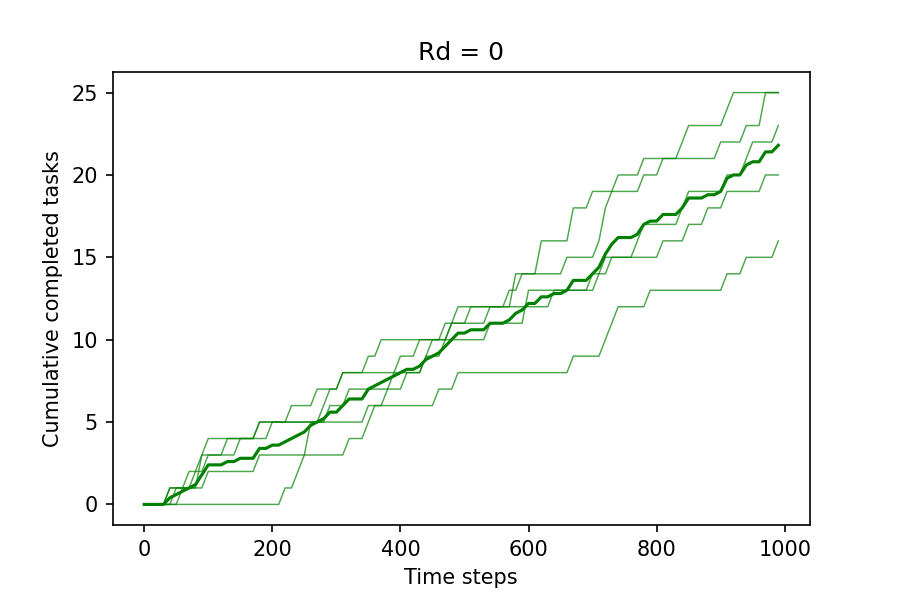
\includegraphics[width=\linewidth]{figures/Rd_0.png}
    \end{subfigure}
    \begin{subfigure}{.5\textwidth}
      \centering
      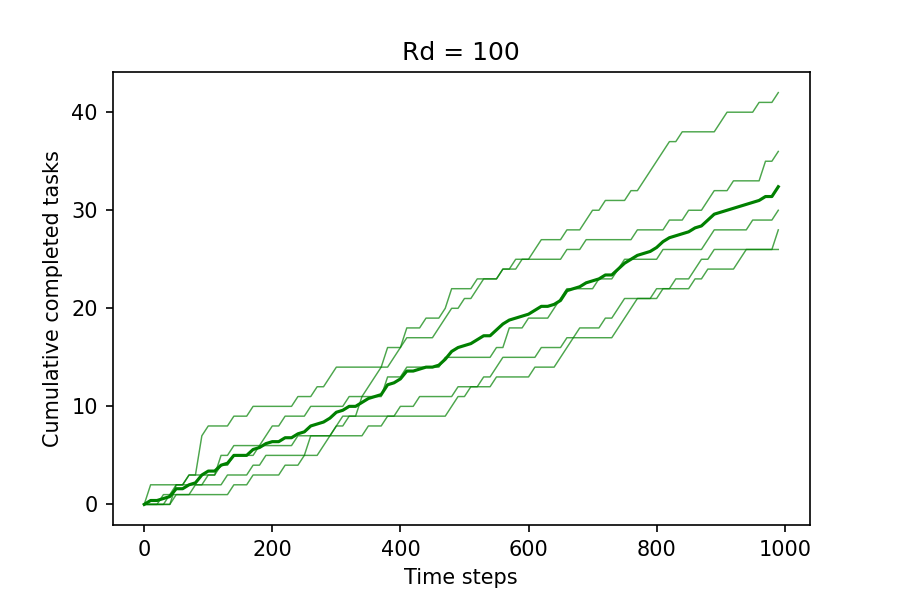
\includegraphics[width=\linewidth]{figures/Rd_100.png}
    \end{subfigure}
\end{figure}

\begin{figure}[ht]
    \begin{subfigure}{.5\textwidth}
      \centering
      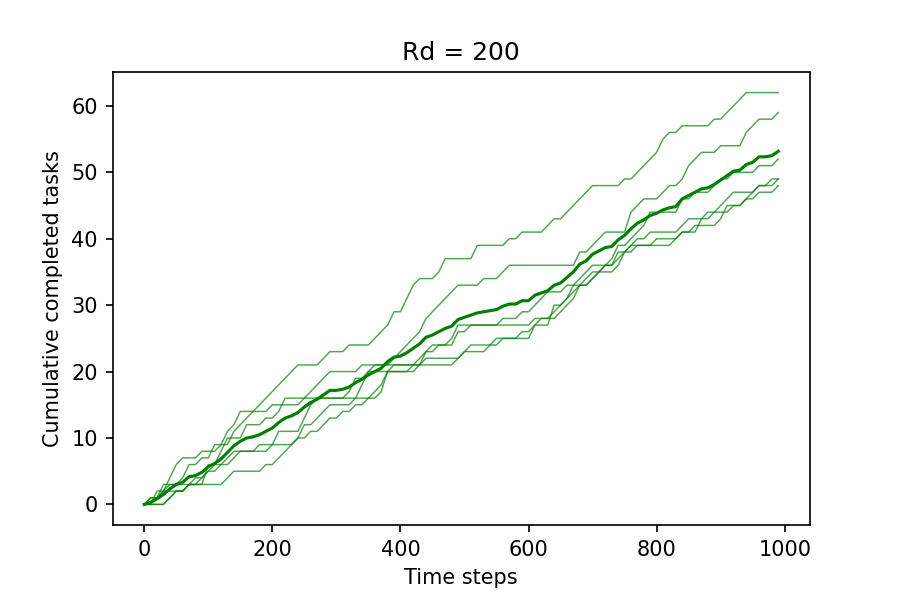
\includegraphics[width=\linewidth]{figures/Rd_200.png}
    \end{subfigure}
    \begin{subfigure}{.5\textwidth}
      \centering
      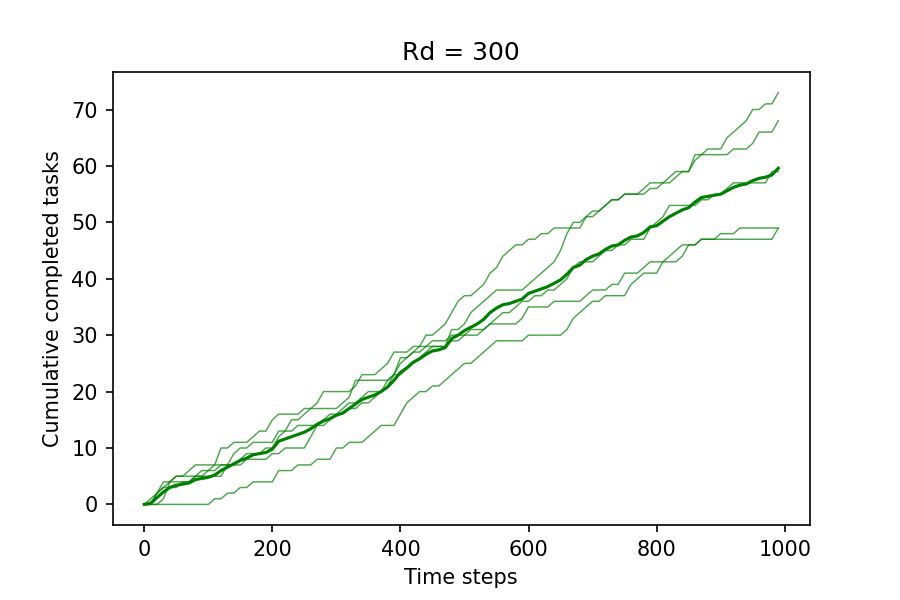
\includegraphics[width=\linewidth]{figures/Rd_300.png}
    \end{subfigure}
\end{figure}

\begin{figure}[ht]
    \begin{subfigure}{.5\textwidth}
      \centering
      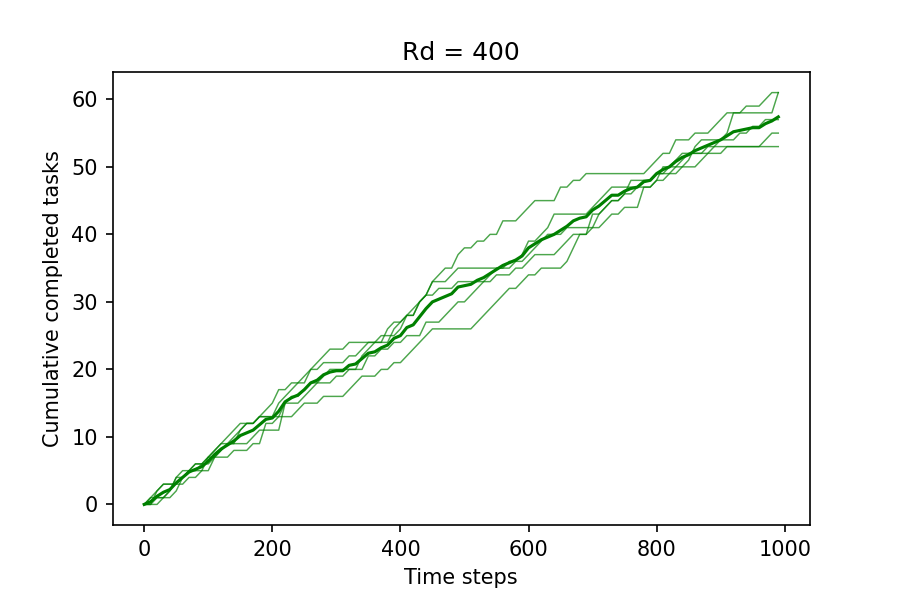
\includegraphics[width=\linewidth]{figures/Rd_400.png}
    \end{subfigure}
    \begin{subfigure}{.5\textwidth}
      \centering
      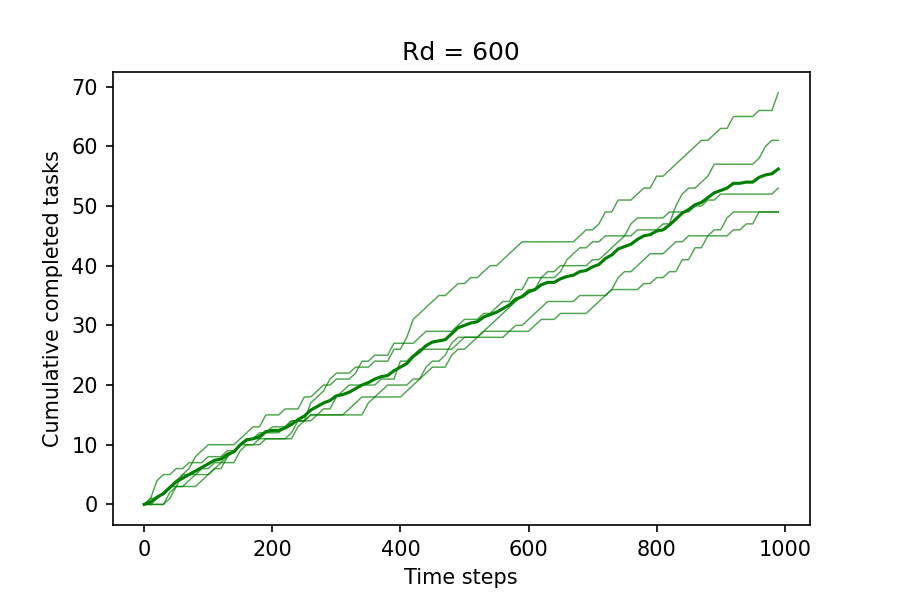
\includegraphics[width=\linewidth]{figures/Rd_600.png}
    \end{subfigure}
\end{figure}

\begin{figure}[ht]
    \begin{subfigure}{.5\textwidth}
      \centering
      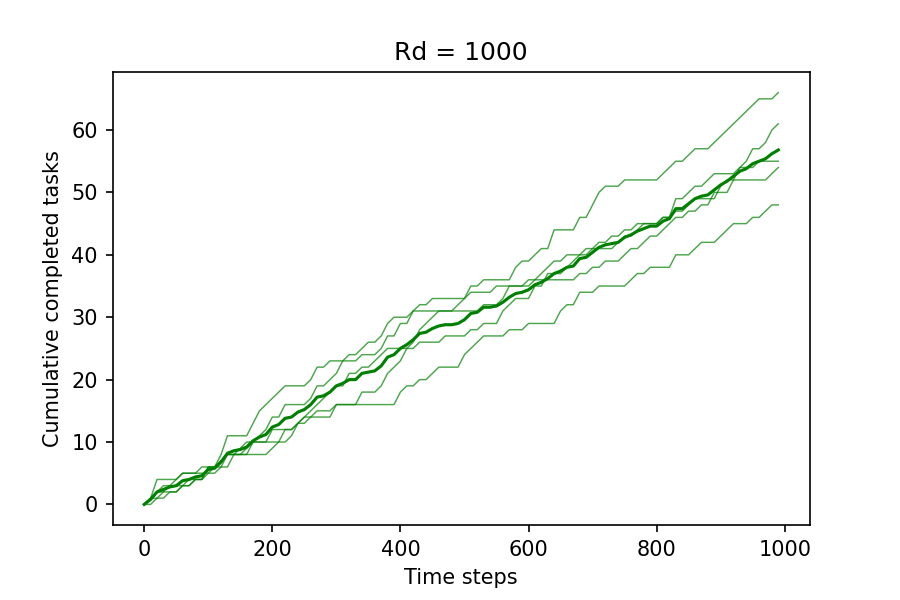
\includegraphics[width=\linewidth]{figures/Rd_1000.png}
    \end{subfigure}
    \begin{subfigure}{.5\textwidth}
      \centering
      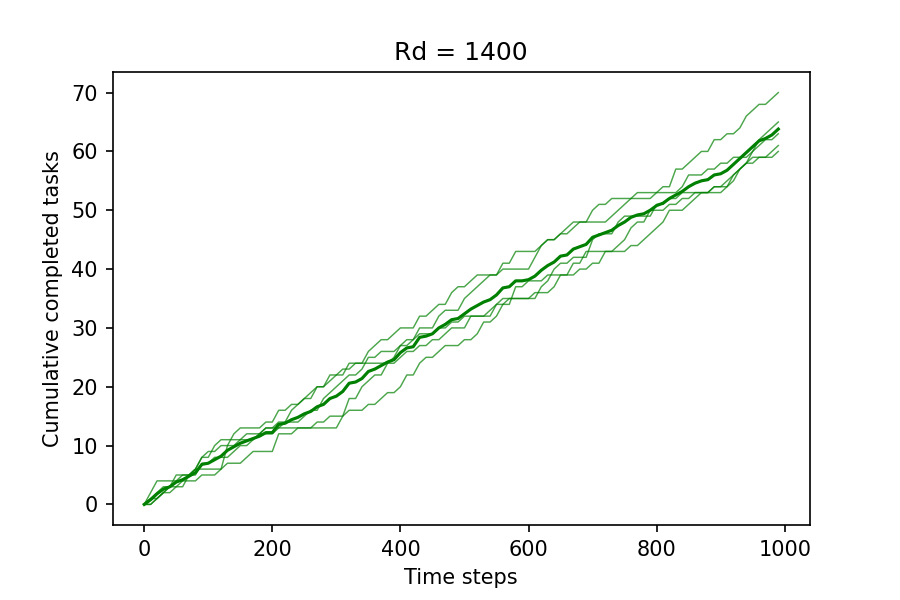
\includegraphics[width=\linewidth]{figures/Rd_1400.png}
    \end{subfigure}
\end{figure}

\pagebreak
\section{Code listing}
\label{app:code}

\lstinputlisting[firstline=0,lastline=280]{../pygame_task_search.py}

\end{document}